\chapter{Methodology}
As previously mentioned, both binary thresholding encoding and deep learning feature map extraction have their downsides. Therefore this thesis proposes to use a combination of both, a segmentation model which can extract classes into their respective SDRs.
\begin{figure}[H]
\centering
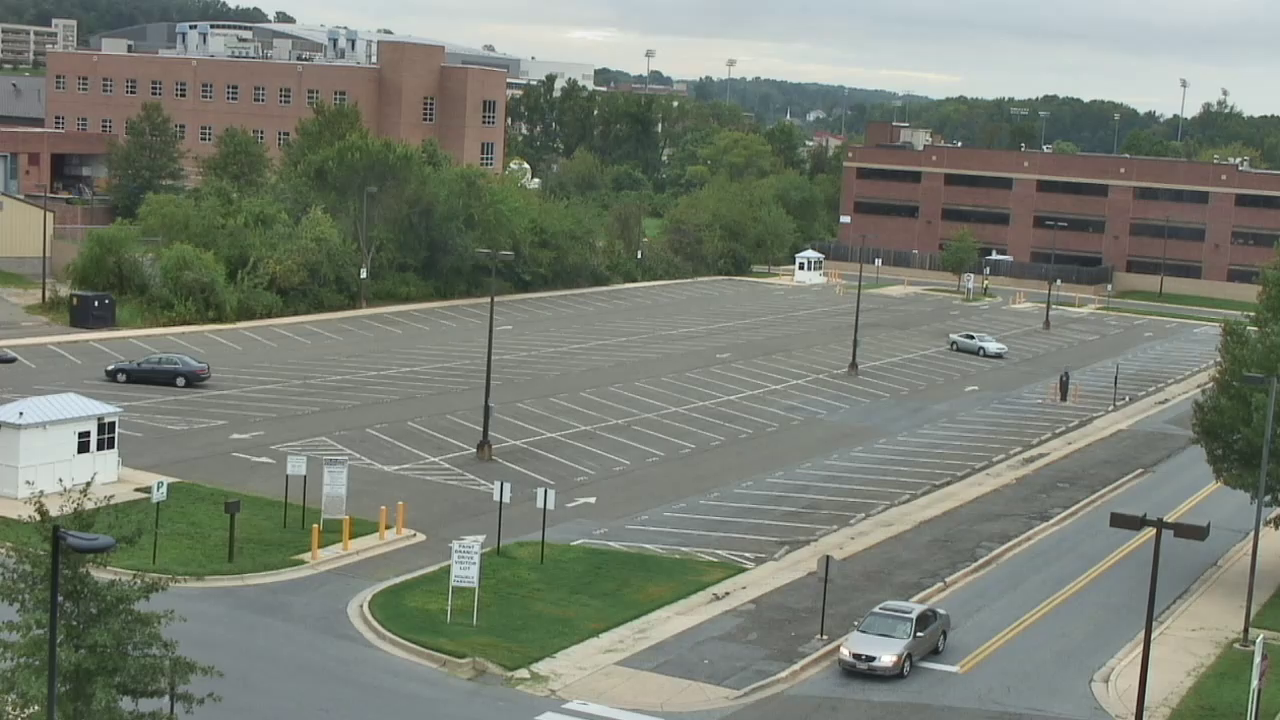
\includegraphics[width=.45\textwidth]{resources/methodology/original.png}\hfill
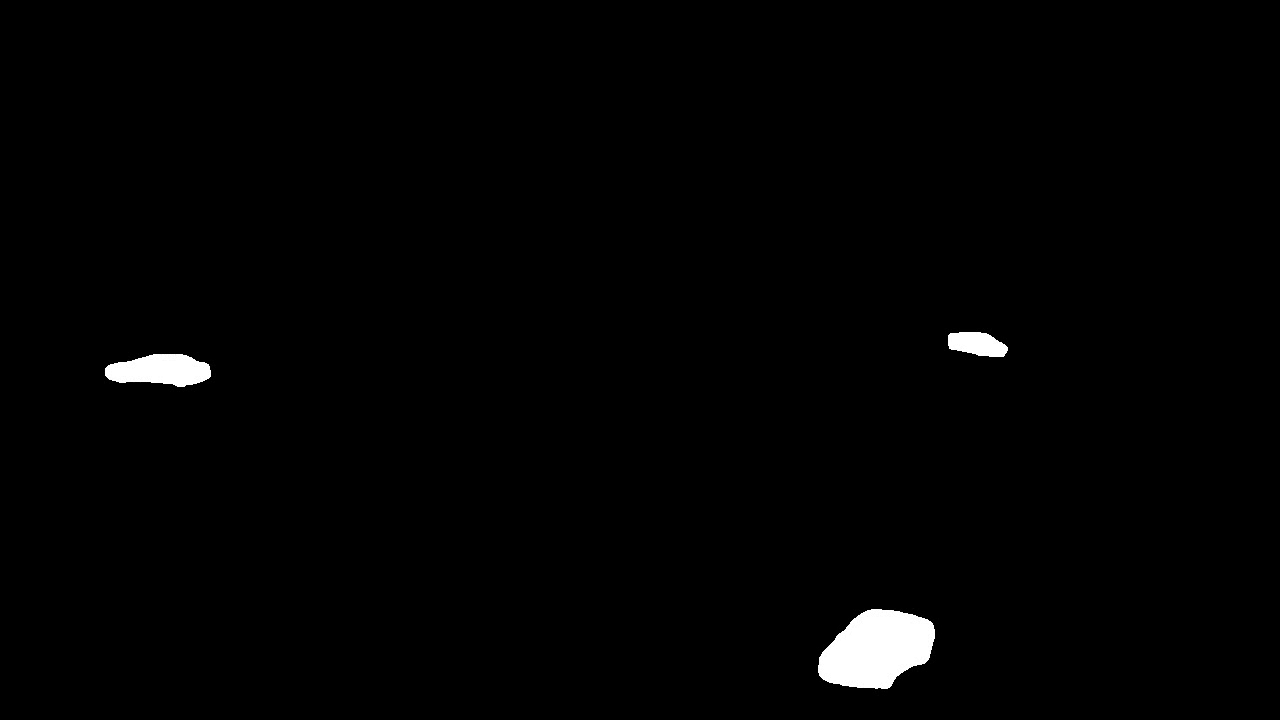
\includegraphics[width=.45\textwidth]{resources/methodology/car_segmentation.png}
\caption{Segmentation result of cars}
\label{fig:figure3}
\end{figure}
The idea is that the SP will learn to find an optimal general representation of cars. How general this representation is can be configured using the various parameters, but ideally they should be set so that different cars will be considered equal while trucks and motorcycles will be different. The task of the TM will then be to learn the common patterns that the cars exhibit, their speed, shape, and positioning will be taken into account. Finally the learning will be set so that new patterns are learned quickly, but forgotten slowly. This will allow the system to quickly learn the norm, even if there is little activity, while still reacting to anomalies.\par
One issue that becomes evident is the lack of invariance. Because the TM is learning the global patterns, it learns that it is normal for cars to drive along the road but only in the context of there being cars parked in the parking lot. It is instead desired that the TM learns that it is normal for cars to drive along the road, irrespectable of whether or not there are cars in the parking lot. This thesis proposes a solution based on dividing the image into a grid, and have a separate SP and TM for each cell in the grid. The anomaly scores of all the cells are then aggregated into a single anomaly score.
\begin{figure}[H]
\centering
\includegraphics[width=0.7\textwidth]{example-image-a}
\caption{The image divided into a grid.}
\label{fig:grid}
\end{figure}
